\section{Introducci\'on te\'orica}

Dado que la modelización utlizada para este problema es un sistema de ecuaciones y que en base a algunos datos que nos dan (posición de las saniguijuelas, dimensiones y temperaturas de los bordes) tenemos que calcular los valores de muchas celdas, lo que hay que resolver es un sistema de ecuaciones. 
Lo primero que se nos viene a la mente cuando tenemos esto es el método de eliminación gaussiano. Este transforma la matriz de coeficientes en una matriz triangular superior y luego mediante back substitution 
se pueden obtener todos sus valores. Si bien este método no funciona siempre veremos que para nuestro caso puede otorgarnos soluciones aceptables.

Veamos ahora más en detalle como funciona cada uno de estos algoritmos.

\subsection{Algoritmo de eliminación gaussiana}

Este algoritmo consisnte en restar multiplos de filas entre sí, comenzando desde la primera, con el objetivo de lograr todos ceros por debajo de la diagonal y numeros disintos de cero en la diagonal, 
es decir una matriz triangular superior. En el caso que me quedase un 0 en la diagonal el algoritmo comprende la opción de pivoteo (mas adelante demostraremos que en realidad no necesitamos) que consiste en intercambiar 
filas entre sí para que esto no suceda.

Veamos ahora algún ejemplo concreto con la siguiente matriz de $3 \times 3$:

\[ \left( \begin{array}{ccc}
4 & 8 & 9 \\
1 & 5 & 2 \\
2 & 3 & 1 \end{array} \right)\] 

Hago 

\emph{F2 = F2 - 1/4 (F1) y F3 = F3 - 1/2 (F1)} 
\[ \left( \begin{array}{ccc}
4 & 8 & 12 \\
0 & 3 & -1 \\
0 & -1 & -5 \end{array} \right)\] 

y ahora

\emph{F3 = F3 - -1/3 (F2) } 
\[ \left( \begin{array}{ccc}
4 & 8 & 12 \\
0 & 3 & -1 \\
0 & 0 & -31/3 \end{array} \right)\] 

Si entendemos la matriz original como un sistema de ecuaciones con 3 variables igualadas a distintos resultados, como podemos ver a continuación:

\[ \left( \begin{array}{ccc}
4x & 8y & 9z \\
1x & 5y & 2z \\
2x & 3y & 1z \end{array} \right)\] 

Con esta nueva matriz triangulada podríamos calcular facilmente el valor de cada variable ya que de la última ecuación podemos despejar facilmente el valor de Z, reemplazarlo en las otras ecuaciones y así calcular las otras variables.


\newpage

Por último cabe destacar que la complejidad computacional de esta trinagulación es de O($n^3$). Lo cual puede llegar a un cálculo sumamente extenso si nuestro n es considerablemente importante. Por esto es que decidimos pensar un poco mas la situación y encontrarle la vuelta para resolver en un tiempo razonable.

\subsection{Matriz banda}

Analizando la matriz del sistema de ecuaciones que se genera a partir de la representación del Parabrisas observamos que presenta las caracteristicas de un tipo de matriz llamada "banda", la cual se distingue por tener todas las celdas en 0 salvo en la diagonal ensanchada, es decir, que p celdas a la izquierda y q a la derecha de la diagonal a lo sumo tienen algunos o todos los valores distintos de 0. En nuestro caso, al construir la matriz nos basamos en el tipo de celda, si es el borde frío o una sanguijuela el coeficiente respectivo sera un 1 en la diagonal igualado a la temperatura correspondiente, pero en el caso de ser una celda vacía en la diagonal irá un -4, a los costados un 1 y representando la fila de "arriba" y "abajo" del parabrisas iran un 1 a "m" columnas de distancia de la diagonal. Finalmente la matriz resultante quedará con una banda de ancho m+m, con "m" el ancho del parabrisas.

Aca podemos ver un ejemplo de una matriz banda:

\begin{figure}[htb]
\begin{center}
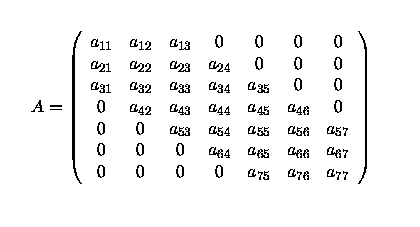
\includegraphics[scale=0.70]{imagenes/matriz_banda.jpg} 
\caption{Matriz banda 7x7} 
\end{center}
\end{figure}







